%; whizzy chapter
% -initex iniptex -latex platex -format platex -bibtex jbibtex -fmt fmt
% 以上 whizzytex を使用する場合の設定。

%     Tokyo Debian Meeting resources
%     Copyright (C) 2007 Junichi Uekawa

%     This program is free software; you can redistribute it and/or modify
%     it under the terms of the GNU General Public License as published by
%     the Free Software Foundation; either version 2 of the License, or
%     (at your option) any later version.

%     This program is distributed in the hope that it will be useful,
%     but WITHOUT ANY WARRANTY; without even the implied warranty of
%     MERCHANTABILITY or FITNESS FOR A PARTICULAR PURPOSE.  See the
%     GNU General Public License for more details.

%     You should have received a copy of the GNU General Public License
%     along with this program; if not, write to the Free Software
%     Foundation, Inc., 51 Franklin St, Fifth Floor, Boston, MA  02110-1301 USA

%  preview (shell-command (concat "evince " (replace-regexp-in-string "tex$" "pdf"(buffer-file-name)) "&"))
% 画像ファイルを処理するためにはebbを利用してboundingboxを作成。
%(shell-command "cd image200708; ebb *.png")

%%ここからヘッダ開始。

\documentclass[mingoth,a4paper]{jsarticle}
\usepackage{monthlyreport}

% 日付を定義する、毎月変わります。
\newcommand{\debmtgyear}{2007}
\newcommand{\debmtgdate}{17}
\newcommand{\debmtgmonth}{11}
\newcommand{\debmtgnumber}{34}


\begin{document}

\begin{titlepage}

% 毎月変更する部分, 本文の末尾も修正することをわすれずに

 第\debmtgnumber{}回 東京エリア Debian 勉強会資料

\vspace{2cm}

\begin{minipage}[t]{0.6\hsize}
\vspace{-2cm}
{\fontsize{60}{60}
{\gt
\color{dancerdarkblue}
東京エリア \\
デビアン \\
勉強会
}}
\end{minipage}
\begin{minipage}[b]{0.4\hsize}
\hspace{-1cm}
\includegraphics[width=9cm]{image200502/openlogo-nd.eps}
\end{minipage}

\vspace{3cm}
\hfill{}Debian勉強会幹事 上川 純一\\
\hfill{}\debmtgyear{}年\debmtgmonth{}月\debmtgdate{}日

\thispagestyle{empty}
\end{titlepage}

\dancersection{Introduction}{上川 純一}


今月のDebian勉強会へようこそ。
 これからDebianのあやしい世界に入るという方も、すでにどっぷりとつかってい
 るという方も、月に一回Debianについて語りませんか?

 目的として次の二つを考えています。

 \begin{itemize}
 \item メールではよみとれない、もしくはよみとってられないような情報につ
       いて情報共有する場をつくる
 \item Debianを利用する際の情報をまとめて、ある程度の塊として整理するた
       めの場をつくる
 \end{itemize}

 Debianの勉強会ということで究極的には参加者全員がDebian Packageをがりがり
 と作るスーパーハッカーになった姿を妄想しています。

 Debianをこれからどうするという能動的な展開への土台としての空間を提供し、
 情報の共有をしたい、というのが目的です。


\newpage

\begin{minipage}[b]{0.2\hsize}
 \colorbox{dancerlightblue}{\rotatebox{90}{\fontsize{80}{80} 
{\gt \color{dancerdarkblue}デビアン勉強会}}}
\end{minipage}
\begin{minipage}[b]{0.8\hsize}
\hrule
\vspace{2mm}
\hrule
\setcounter{tocdepth}{1}
\tableofcontents
\vspace{2mm}
\hrule
\end{minipage}

\dancersection{事前課題}{上川 純一}

今回の事前課題は
「Debian の Live CD ってこんなふうに使ってます」もしくは「ノートPCやデスクトップPCではなく、サーバ機器での Debian に期待するものって何?」というタイトルで200-800文字程度の文章を書いてください。というものでした。
その課題に対して下記の内容を提出いただきました。

\subsection{前田 耕平}

\subsubsection{「ノートPCやデスクトップPCではなく、サーバ機器での Debian に期待するものって何?」}
完全な最小構成のインストーラですね。Debianでもやっぱり最小構成でインストールしても無駄なパッケージが多いので、サーバを構築するときは必ず最小構成でインストール後にさらにそこから引っこ抜いています。
Sargeに比べたらEtchは結構良くなったと思いますけど、まだ足りない、もとい多いですね。
RHELとかSUSEなんて多すぎて論外ですけど。

\subsubsection{「Debian の Live CD ってこんなふうに使ってます」}
DebianのLive CDは正直使ったことはありません。Live CDは、重いですけどKNOPPIX使ってます。
USB-KNOPPIXなんかも使っていたりしますが、CD-ROMよりは軽いです。
KNOPPIXがもともとDebianベースだと言っても、APT使わなければ意味ないですね。
使い方としては、やっぱりIAサーバのメンテナンスや、期間が短いテストを行うときに使っています。

\subsection{satoken}

\subsubsection{ノートPCやデスクトップPCではなく、
サーバ機器での Debian に期待するものって何?}

\begin{description}
 \item[安定性]
  多少古くても安定していて欲しい....と言う点でDebianは良さそう
  でも、本当にそうだろうか? そうだと思いたいんだけど...

 \item[構築容易性]
  Installしてから動かす迄に必要な設定が少なくて済む。
  依存性を考慮して必要な物はついでに入れてくれるし。
  他のディストリビューションでは設定作業量が何かと多い気が...

 \item[パッケージ管理]
  aptに感動。
  ところで、apt-cacherの話は?ありますでしょうか?期待してます。
 (apt-proxyが落ちやすいので)
\end{description}

期待したいんだけど期待できない点

\begin{description}
 \item[最新ハードウェア対応]
  Ubuntuからのフィードバックで加速されるかなぁ〜?

 \item[有償ソフト対応]
  「Debianでも動く」と言ってくれるソフトがとても少ない。
  DELLがUbuntu搭載PCの日本語版を出してくれれば.....
\end{description}


 と言う感じで、Ubuntuが流行ればDebianにも良い影響が
波及してくるのでは?と期待してます。


\subsection{jun araki}
\subsubsection{サーバ機器での Debian に期待するものって何?}

サーバ機器の場合、まず OS としての安定性(可用性)とセキュリティを期待します。
それぞれ Debian について考えてみますと、以下のような点が強みとして挙げられると思います。

\begin{itemize}
 \item  安定性(可用性)
	\begin{itemize}
 \item  sid, testing, stable といったリリースサイクルによる厳格なテストと品質管理
 \item  高可用性を実現する為のパッケージ(Idirectord
 \footnote{ldirectord, \url{http://www.vergenet.net/linux/ldirectord/}},
  Ultra Monkey
 \footnote{Ultra Monkey, http://ultramonkey.jp/} など)が提供されていること
	\end{itemize}

 \item  セキュリティ
\begin{itemize}
 \item  ML によるセキュリティ関連のアナウンス
 \item  上記のテストや品質管理をベースとしたセキュリティアップデート
\end{itemize}
\end{itemize}
 これら以外には、サーバ管理やインストールの容易性を期待します。

 サーバ台数が増えてくると、ハードウェアの故障件数も増えてきますので、
 OS の比較的頻繁な入れ替えやバージョンの異なる OS を(一時的に)共存
 させた状態での運用といったことも想定されます。

 それに対して、Debian の場合サーバ管理については、

\begin{itemize}
 \item  FHS(File Hierarchy Standard)準拠による透過性
 \item  自動化ツール群の豊富さ
\end{itemize}

といったところが特徴かと思います。\footnote{"The Debian System --- その概念と技法"}
ツールの方はまだそれほど使いこなしてはないのでこれから試してみます。

インストールについては、これもまだ使ったことがないのですが、 preseed
による自動インストールというのがあります。ただ、既存のパーティションを
利用できない(パーティションを再作成するか空き領域を利用するかしかない)
といった制限があるようです。\footnote{ "Debian GNU/Linux インストールガイド B.1.2. 制限",
\url{http://www.debian.org/releases/stable/mipsel/apbs01.html.ja\#preseed-limitations}}

\subsection{山本 琢}

\subsubsection{Debianにサーバとして期待すること。}

\begin{description}
 \item[シェルスクリプトを書かずに管理できるようにしたい]
	    今のLinuxは敷居が高いと思う
 \item[kickstart(自動OSインストール)のサポート]
	    一度に複数の同一形式PCにインストールしたい
 \item[各種ログ出力のカスタマイズが容易に出来ること(syslog-ngのカスタマイズ)]
	    ログ出力設定が難しい
 \item[TOMOYO(若しくはAppArmor)のサポート]
	    セキュリティー管理をSELinux以外の選択肢が欲しい
 \item[DBレプリケーション設定のGUI化(dpkg-reconfigureのようなもの)]
	    Debianの管理ツールで容易に設定出来ると嬉しい
\end{description}


\subsection{Hajime Fukuda}

\subsubsection{「ノートPCやデスクトップPCではなく、サーバ機器での Debian に期待するものって何?」}

僕がサーバでDebianを使っている理由として、最小構成でのインストールが容易で、またaptをつかえば簡単に新しいパッケージを入れられるということがある。サーバではなるべく余計なものを入れないということが基本であるので、Debianのこの性格はサーバにとても適していると思う。
また、Debianでは、サーバの設定は基本的にviなどで設定ファイルを手で編集して適用する。他のディストリビューションではなんだかGUI設定ツールがたくさんついているが、サーバにXは不要だし、こみいった設定などはやはりファイルを直接編集した方がやりやすいと思う。僕はこういったところもDebianをサーバに選ぶポイントにしている。

\subsection{小林 `nori1' 儀匡}

\subsubsection{「Debian の Live CD ってこんなふうに使ってます」}

Live CDと言えるのか微妙ですが、インストーラCDをレスキュー用に使っています。

また、ぼく自身は使ったことはないのですが、何年か前に、GNU/Linux環境に
慣れていないWindowsユーザが統計言語 GNU R など研究者に有用なソフトウェ
アを手軽に使用できる方法としてKnoppixがよく紹介されていた覚えがありま
す (今でもそうかもしれませんが、今だとCygwin上でX環境を構築するのも楽
でしょうし、そもそもCygwinさえ通さずにWindowsネイティブアプリケーショ
ンとして使えるFLOSSソフトウェアも増えているので、前ほどは重要性は減っ
ているのではないかと思います)。インストールさえ敷居が高い (手を出しに
くい)、というユーザはいるはずなので、ライブ CD は重要だと思います。

\subsubsection{「ノートPCやデスクトップPCではなく、サーバ機器での Debian に期待するものって何?」}

最小構成でインストールでき、必要なものは追加で簡単にインストールできる
こと、でしょうね。その意味でDebianは間違いなく他のディストリビューショ
ンに勝っていると思いますから、今後もその路線は維持していただきたいです。
また、ネットワークインストールによって複数のマシンに同じような環境を簡
単にセットアップできることも重要だと思いますが、ぼくは企業のような大規
模な組織でのシステム管理経験はないので単なる推測に過ぎません。


\subsection{Hideki Yamane}

\subsubsection{「ノートPC やデスクトップPC ではなく、サーバ機器でのDebian に期待するものって何?」}
 もっと簡単なセットアップが出来るといいですよね。
 Windows Server 2003 の様に「○×サーバ機能」を選ぶと、ウィザードでサクッ
と入ってしまうとか。

\begin{commandline}
 ------------------------------------------------
 |  導入したいサーバ機能を選んでください
 |
 |   - LAMPサーバを纏めて導入
 |
 |   - web サーバ (apache, lighttpd)
 |   - ファイルサーバ (Samba, NFS)
 |   - DNS サーバ (bind)
 |   - DHCP サーバ (dhcp3)
 |   - LDAP サーバ (openldap)
 |   - Radius サーバ (xxx)
 |   - NTP サーバ (ntpd)
 ------------------------------------------------
\end{commandline}

 みたいな感じでさくさくできるの。

\subsubsection{「Debian のLive CD ってこんなふうに使ってます」}
 live-helper 使って遊んでるだけですね。もう少し楽になるように要望を出していくつもりです。

\subsection{hiro}

\subsubsection{Debian の Live CD ってこんなふうに使ってます}

Debianと直接の関係はありませんが、先日gOSを使ってみました。

\subsubsection{ノートPCやデスクトップPCではなく、サーバ機器での Debian に期待
するものって何?}

安定性と長期のサポート。以前Fedora Coreを使用していた際、パッケー
ジのアップデートをしただけでSambaのメジャーバージョンが上がって
しまい、焦ったことがあります。またサポート期間が短いと頻繁に新し
いものへ移行しなければならず、止めづらいサーバへの導入は苦しいも
のがあります。

\subsection{山本 浩之}

\subsubsection{「Debian の Live CD ってこんなふうに使ってます」}

使っていません(わら
KNOPPIX ならちょこっと使っています。
主にハードディスクエラーが出たときの fsck で使っております。
あと、パーティションを切るときに使いました。

これでは課題にならないので、こんな Debian Live CD があったらいいな、を書
きます。
CD から HDD のメンテナンスするときは、基本的に、HDD のパーティションをど
こかにマウントし、そのマウントしたディレクトリに chroot した後、HDD 内の
コマンドを使うのが一般的ですよね。
そこで、ディスクエラーなどで HDD の dpkg コマンドや apt コマンドなどの基
本的なコマンドが壊れても修復できるような、メンテナンス専用 Live CD があ
るといいです。
具体的には CD 内に存在する apt コマンドとかで HDD のパーティションに直接
パッケージ (例えば dpkg パッケージとか) がインストールできる、そんな CD
があると嬉しいです。


\subsubsection{「ノートPCやデスクトップPCではなく、サーバ機器での Debian に期待するも
のって何?」}

サーバ機器は使ってないので、あまり具体的にイメージできないのですが、一般
的には新しいパッケージより安定したパッケージを採用ってことになりますかね?
あと、24 時間稼働させるとなると、消費電力と熱のコントロールも必要になり
ますかね?
処理速度重視より、安定にエラー無く稼働することが重視されると思います。

ついでに、oldstable のセキュリティサポート期間が、現在、次の stable がリ
リースされて約一年ってことになっています。
今のところ、stable リリースのサイクルが約一年半に一度が良かろう、と言わ
れているそうですが、この残り半年間のため、一つ飛ばしの dist-upgrade がで
きないでいます。
セキュリティサポートの期間を次の次がリリースされるまでに伸ばしたら、
stable の一つ飛ばしができ、助かる人もきっとたくさんいるのではないかと思
います。

\subsection{kita-san}

\subsubsection{Debian の Live CD ってこんなふうに使ってます}

  「Live CD」といえば、これまで「Knoppix」を使っ
ていたのですが、この課題で「Debian」純正(?)の
「Live CD」があるのを思い出しました。

  では早速使ってみよう……、と言う事で Google で
情報収集………?! 「livehelper」なにそれ!
ISOイメージとかないんですかぁ? こりゃだめだ!

  ということで、勉強会で岩松さんの「live-helper
ネタ」を聴いて勉強させていただきます。

  そんなわけで、お題の回答は「まだ使っていません」
ということで、スミマセン!

%%% trivia quiz
\dancersection{Debian Trivia Quiz}{上川 純一}

ところで、みなさん Debian 関連の話題においついていますか?Debian関連の話
題はメーリングリストをよんでいると追跡できます。ただよんでいるだけでは
はりあいがないので、理解度のテストをします。

今回の出題範囲は\url{debian-devel-announce@lists.debian.org} に投稿された内容からです。
\begin{multicols}{2}
 
 \subsection{問題}

 \santaku
 {10/4 にアナウンスがあった alioth のサービスに追加されたものは?}
 {VSSサポート}
 {darcsサポート}
 {p4サポート}
 {B}
{}

 \santaku
 {DebianGisチームは何をするチームか?}
 {Gisのパッケージのメンテナンス}
 {DebianをGisでのっとるプロジェクト}
 {人間関係をギスギスしてみる}
 {A}
{}

 \santaku
 {testing security のメールの仕組みで何がかわったか}
 {unstable から testing へのマイグレーションでセキュリティーバグが修正さ
 れてもアナウンスされるようにした}
 {昨年度 Debian testing security team がCVEを5500も処理したことが自慢できるようになった}
 {SMTPプロトコルのハンドシェークが変わった}
 {A}
{}

 \santaku
 {Debconf8 の日程は}
 {5月1日から5月10日}
 {8月2日から8月17日}
 {12月24日から1月1日}
 {B}
{}

 \santaku
 {http://security-tracker.debian.net/tracker/ で何が見れるか}
 {手元のマシンが脆弱化どうかの試験}
 {セキュリティーについての入門}
 {セキュリティーバグの現在の状態}
 {C}
{}

 \santaku
 {Debian System Administrator として新しく任命されたのは誰か}
 {Sven Luther}
 {Phil Hands}
 {Peter Palfrader}
 {C}
{}

 \santaku
 {ries.debian.org (ftp-master) はどれくらい停止していたか}
 {11月5日から11月12日}
 {11月5日から11月30日}
 {11月1日から11月5日}
 {A}
{}
\end{multicols}

\dancersection{最近のDebian関連のミーティング報告}{岩松 信洋}

\subsection{東京エリアDebian勉強会32回目報告}
% (query-replace-regexp "<.*?>" "")
% (query-replace-regexp "^[ 	]*" "")


まず小室さんに exim の簡単な情報、設定方法、exim-jpの活動について話してい
ただきました。exim は他のMTAと比べると、設定が容易にでき、他のアプリケー
ション( ClamAV など)の連携も簡単で、1行で使用可能になるところが魅力的に
感じました。exim のマニュアルは 3万行あるとのことです。3万行の英語から 特
定の情報を取り出すのは大変なので、ユーザーのために exim-jp で翻訳している
とのことです。また、簡単なチュートリアルや、他のMTAのとの比較があれば導入
しやすくなるので、そちらも平行展開していくのがいいのではないか、という意
見がありました。

その次にあまり知られていない apt-xxx について岩松が話しました。10個ほどの
apt-xxx について簡単に説明をしました。どれもあまり使われていない/存在すら
しらない ということがわかりました。その中で、apt-proxy / apt-cacher 、
apt-transport-https について、興味がある方が多かったです。今後の勉強会で
取り上げられることがあるかもしれません。期待です。

最後に「あなたがDebianで使っている MTA のこだわりの設定」もしくは
「Debian で利用しているこんな便利な/楽しいメッセージツールあるいは日頃使っ
ていて気にかかるメッセージ関連ソフトのこの部分」として事前課題を提出して
いただき、ディスカッションを行いました。

Postfix を使っている方が多く、日本語での情報が多いことがキーになっている
ようです。しかし、設定ファイルを記述するのがけっこうめんどうくさいという
意見がありました。小室さんの発表してくれた exim では容易に設定できるよう
なので exim 魅力を感じている人が増えたような気がします。

帰り際に青木さんが im-switch の実装のための インプットメソッドの 調査をし
ました。Debianでは多くの入力用ソフトウェアが存在するのですが、インプット
メソッド 切り替え用の フロントエンドである im-switch の整備を行うためです。
後藤さんが出してくれた現在のインプットメソッド環境は複雑になっているので、
IM-BUSの実装に期待です。


\subsection{東京エリアDebian勉強会33回目(OSC Tokyo/Fall 出張会議)報告}
% (query-replace-regexp "<.*?>" "")
% (query-replace-regexp "^[ 	]*" "")


武藤さんのセミナーは30人部屋が満員になる盛況だったそうです。CUPSの話を
UNIX系OSでの印刷機構とCUPSの現状についての話でした。Q\&Aのセッションでは、
バイナリドライバは問題が多いということに帰着しました。

山根さんのミニセミナーも盛況だったようです。会場のホワイトボードにはって
あった質問に回答(というよりつっこみ)をしていました。

ブースでの展示ではML350G5でDebianが稼働しており、 WebCam(EyeToy)が稼働
しているところ、ML110G4でDebianが稼働しているところ、WS003SH(りざぽん)
上でDebianが稼働しているところ、 USL5PでDebianが稼働しているところを展
示しました。組み込みガジェット系の展示が興味を引いたようです。サーバ系
は淡々と展示していました。 エンタープライズ系でDebianを利用したいという
方もいらしたようです。

ブースでホワイトボードを設置し、そこにメッセージを書いてもらうという企
画を実施しました。 もらったメッセージは次です:
\begin{multicols}{2}
 
 \begin{itemize}
    \item パッケージみつけれません
    \item パッケージメンテナになりたいのですが
    \item コマンドからパッケージ見つける方法おしえてー
    \item apt-proxy のディレクトリに手動でパッケージファイルをおいてもよいの?
    \item Debianをつかっていると仲間外れも気にならなくなりました
    \item いつかいれようとおもっているんですけどねー。FD起動でインストールできるディストリも少なくなりましたし。
    \item etchな人、好きです。
    \item SELinuxは入るのですか?
    \item 今etch使っています。etch の次の名前は?
    \item OpenBlockS266 6台でDebian 毎日元気に稼働中です。
    \item Etch使ってます。
    \item すきです。
    \item lenny いつ stable になりますかね。
    \item これからさわってみたいとおもいます。
    \item 会社のsidマシンをなんとかしたい。
    \item experimental なパッケージをいれて不安定になりかけた(人柱的な意味で)
    \item IntelのMB 965RYにDebianが入りません、鬼門ですから気をつけてください。
    \item W-zero3がすごい、次は [es] にも
    \item さすがDebian!w-zeroで動くなんて好きになりそうです。
    \item DebianだったらZERO3[es]も活用できるかも。
    \item Debian使ってます、W-zero3すごい、今度、勉強会でます。
    \item 参上
    \item lenny と etch 使ってます!!
    \item etchですぐ使える USB Web カメラを教えてください。
    \item aptってラクです。
    \item DEBIANでEXIM使うとHappyになれます
    \item Zaurusもネイティブで動かしたいな
    \item 非力なリブレットでもサーバとしてサクサク動くので助かってます。
 \end{itemize}
\end{multicols}


懇親会は蒲田の二葉で実施しました。 武藤さん、野首さん、小室さん、本庄さ
ん、山根さん、あけどさん、鈴木(LSS)さん、 樽石さん、山本さん、上川で
した。 また、遅れて榎さんが参加しました。 今日の宴会は昔話がすぎるぞと
いうことを反省して終了しました。

 \begin{figure}[H]
 \begin{center}
  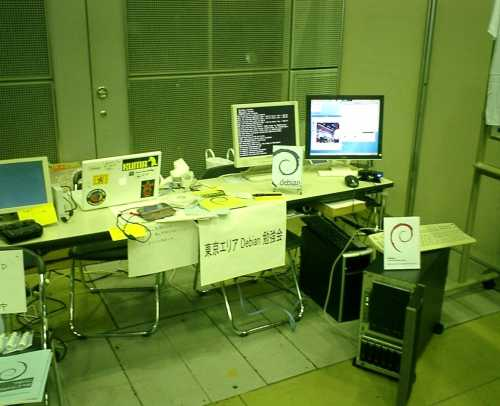
\includegraphics[width=0.4\hsize]{image200710/booth.jpg}
  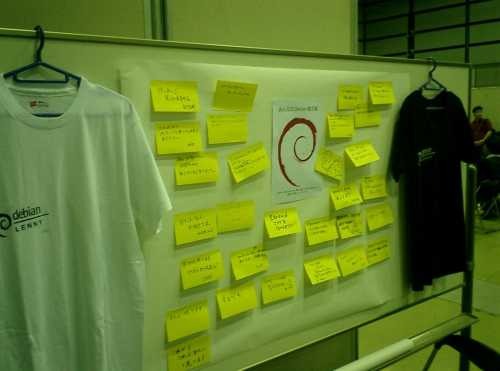
\includegraphics[width=0.4\hsize]{image200710/whiteboard.jpg}
 \end{center}
 \caption{ブースの様子}
 \label{fig:oscfalldebbooth2}
 \end{figure}

展示ブースでの機器の管理について課題があり、いくつか紛失した機材や、まち
がった相手に返却しようとして先方が気づいてかえってくるというケースがあっ
たようです。今後の対策として誰が管理している道具なのかを明記しておく必要
があるかもしれませんね。


\subsection{関西オープンフォーラム報告}
% (query-replace-regexp "<.*?>" "")
% (query-replace-regexp "^[ 	]*" "")

11月10日に関西オープンフォーラム\footnote{\url{http://k-of.jp/}}が開催さ
れ、関西 Debian 勉強会が出展しました。

展示と、セミナーとミニセミナーを実施しました。

6Fの大会場での展示に参加したのは山下さん、のがたさん、川江さん、倉敷さん、名村さん、
清野さん、山根さん、上川の8人でした。Debian のデモ、Debian ステッカーの
販売、DVDの配布、Debian 勉強会冊子の販売を実施しました。

ミニセミナーは山根さんが「Livehelper3分クッキング」として実施しました。
livehelper の料理方法を臨場感たっぷりに説明し、大盛況でした。

セミナーは9F会議室で実施しました。のがたさんとたかやさんが初心者向けの説
明として、aptitude と synaptic の説明をしました。


\subsection{Biella Coleman 宴会}

11月14日、New York University の Biella Coleman と Aram Sinnreich、
Creative Commons の Asheesh 、そして Debian JP の knok、mhatta、dancerj
で宴会をしました。会場は銀座の「がんこ」。DebianのNMプロセスについて、
Debianはオープンだがエリート主義か、ポピュリストかどうかということで激論
をかわしました。

\dancersection{live-helper}{岩松 信洋}
\label{live-helper}
\index{live-helper}
\subsection{live-helperとは}
live-helper は Debian の Live-CD / USBboot イメージを作成するための
ツールです。
作成するためのスクリプトが各種用意され、Live-CD の仕組みを知らない人でも容易
に Live-CD を作成することができます。

\subsection{コマンド}
live-helper はlh\_xxx という形式でコマンドが提供されています。
たくさんのコマンド\footnote{2007/11/02 現在で、67個}が用意されていますが、
基本的に使用するのは、
\begin{itemize}
  \item lh\_config
  \item lh\_build
  \item lh\_clean
\end{itemize}
です。他のコマンドは細かい設定を行うためや、内部処理で使用されます。

\subsection{雛型の作成}
まず、lh\_config コマンドを使って、Live-CD の雛形を作成します。
\begin{commandline}
% lh_config
\end{commandline}

{\bf lh\_config} 実行時にオプションを指定することにより、さまざまな設定を
行うことが可能です。
また、これらのオプションは環境変数としても指定することができます。
例えば、{\bf --union-filesystem} というオプションがあるのですが、この場合は
\begin{commandline}
LH_UNION_FILESYSTEM
\end{commandline}
として、設定することが可能です。
% 環境変数と、オプションで指定した場合の有線順位はどちらが高いか調べること

\subsection{作成された設定ファイルの説明}
lh\_config を実行した後、config ディレクトリ以下に以下のディレクトリが作成されます。
\begin{center}
\begin{tabular}{|c|c|}
\hline
ディレクトリ名 & 説明 \\ \hline \hline
binary & 作成される Live-CD イメージに関する設定が書かれています。\\ \hline
bootstrap & Live-CD 作成環境に関する設定が書かれています。\\ \hline
chroot & Live-CD のユーザーランドに関する設定が書かれています\\ \hline
common & live-helper の基本設定が書かれています。\\ \hline
source & source イメージに関する設定が書かれています。\\ \hline
\end{tabular}\\
\end{center}

これらの設定はテキストファイルになっています。なので、適当なエディタで編集可能ですが、
実際には {\bf lh\_config} コマンドを使い、設定ファイルを書き換えます。


\subsection{細かい設定方法}
live-helper は雛形を作成し、作成された各設定ファイルに追記することによって
細かいカスタマイズが可能になっています。以下にカスタマイズの方法について説明します。

\subsubsection{アーキテクチャの指定}

lh\_config の -a オプションを使用することによって、
作成する Live-CD イメージのアーキテクチャを指定することができます。

\begin{commandline}
% lh_config -a アーキテクチャ名
\end{commandline}

\subsubsection{ディストリビューションの指定}
lh\_config -d オプションを使用することにより、作成する Live-CD のディストリビューション
を指定することができます。

\begin{commandline}
% lh_config -d ディストリビューション名
\end{commandline}

\subsubsection{言語の指定}
lh\_config -l オプションを使用することにより、Live-CD で使用するデフォルトの言語を設定
することができます。
例えば、デフォルトの言語を日本語にする場合は
\begin{commandline}
% lh_config -l ja
\end{commandline}
とします。

\subsubsection{ブートローダーの指定}
lh\_config の --bootloader オプションを指定することにより、Live-CD で使用する
ブートローダーを指定することができます。

\begin{commandline}
% lh_config --bootloader grub
\end{commandline}

指定することができる ブートローダーは以下の3つです。
\begin{itemize}
\item grub
\item syslinux
\item yaboot
\end{itemize}

\subsubsection{作成するイメージの指定}
live-helperでは、
\begin{itemize}
\item iso 

ISO9660 イメージ
\item net

NET ブート用イメージ 
\item tar 

tar 形式でまとめたもの

\item usb-hdd

USBメモリやUSB-HDD で起動することができるイメージ

\end{itemize}
のイメージを作成することができます。

lh\_config の --binary-images\footnote{-b でも可能} 
オプションを指定することにより、作成するイメージを指定することができます。

\begin{commandline}
% lh_config --binary-images iso
\end{commandline}

\subsubsection{bootstrap および live-image 内で使用する apt-line の変更方法}
live-helper で使用する apt-line は
\begin{itemize}
\item Live-CD 作成に使用する apt-line
\item Live-CD 内の /etc/apt/sources.list に書き込まれる apt-line
\end{itemize}
の2種類があります。

これらは特に指定しない場合、
\begin{commandline}
http://ftp.debian.org/debian/
\end{commandline}
が指定されています。

変更する場合は {\bf lh\_config} コマンドを利用して変更します。
その他に以下の オプションを指定することによって各々の apt-line を変更する事ができます。

\begin{itemize}
\item --mirror-bootstrap-security URL

Live-CD 作成時に使用する セキュリティアップデート向け apt-line を設定します。 
\item --mirror-bootstrap URL

Live-CD 作成時に使用する apt-line を設定します。
\item -m \verb+|+ --mirror-binary-security URL

Live-CD 内で設定される、セキュリティアップーデート向け apt-line を設定します。
\item --mirror-binary URL

Live-CD 内で設定される、 apt-line を設定します。
\end{itemize}


\subsubsection{Debian パッケージの追加}
Live-CD に Debian Project で配布されているパッケージを追加したい場合は、
\begin{commandline}
lh_config --packages "パッケージ名"
\end{commandline}
を実行します。パッケージ名のところは、スペースで区切り、複数パッケージを指定することが可能です。

この方法でパッケージの追加を行った場合、再度実行してしまうと、上書きされてしまうためパッケージの
追加ができません。\footnote{エディタで編集すれば対応できますが。}

複数パッケージの追加や、パッケージの種類のよって管理したい場合は
\begin{commandline}
config/chroot_local-packageslists/
\end{commandline}
ディレクトリに適当なファイルを作成し、パッケージ名を列挙します。
例えば、 bluetooth
\footnote{http://packages.debian.org/sid/bluetooth} メタパッケージを追加したい場合は、

\begin{commandline}
% cat config/chroot_local-packageslists/bluetooth
# bluetooth packages
bluetooth
\end{commandline}
として、パッケージ名をファイルに列挙します。

ファイル名は管理しやすい名前にしておくといいでしょう。

\subsubsection{オリジナル Debian パッケージの追加}

自分で作成した Debian パッケージや オリジナルのパッチを当てた Debian
パッケージは以下の方法で Live-CD に追加することができます。

まず、自分で作成したパッケージ用のレポジトリを作成します。
次に
\begin{commandline}
config/chroot_sources/適当なファイル名.bootstrap
\end{commandline}
を作成し、作成した レポジトリを apt-line として追記します。

\begin{commandline}
config/chroot_local-packageslists/
\end{commandline}
に適当なファイルを作成し、追加したいパッケージ名を書きます。

これにより、Live-CD 作成時に 作成した apt-line からパッケージがダウンロード
され、インストールされます。

作成したapt-line を Live-CD にも追加する場合は
\begin{commandline}
config/chroot_sources/適当なファイル名.binary
\end{commandline}
を作成し、作成した レポジトリを apt-line として追記します。

\subsubsection{apt-line を使わない Debian Package の追加方法}
\begin{commandline}
config/chroot_local-packages/
\end{commandline}
ディレクトリに Debian パッケージをコピーします。
コピーしておくことにより、自動的にLive-CD 内にインストールされます。
依存関係は解決してないので、必要なパッケージは別途 apt を使ってインストール
するように設定しておく必要があります。

\subsubsection{すでに用意されているパッケージリスト}
live-helper ではまとまった環境がパッケージリストとして用意されています。
これらを使用することによって、ある程度容易に Live-CD を作成することが
できるようになっています。
パッケージリストは
\begin{commandline}
/usr/share/live-helper/lists/
\end{commandline}
にあり、これらを利用することが可能です。
これらのリストを利用するには、{\bf lh\_config} オプションの {\bf --packages-lists | -p} 
を使用します。
gnome-desktop ベースの Live-CD を作成する場合、
\begin{commandline}
% lh_config -p gnome-desktop
\end{commandline}
とします。

\subsection{ホスト名を変更する}
Live-CD のホスト名を変更するには、
lh\_config の --hostname オプションを使用します。
\begin{commandline}
% lh_config --hostname myhostname
\end{commandline}
を実行し、設定したいホスト名を指定します。

\subsection{ユーザー名を変更する}
Live-CD に新しいユーザを追加するには、
lh\_config の --username オプションを使用します。
\begin{commandline}
% lh_config --username myname
\end{commandline}
を実行し、追加したいユーザ名を指定します。
パスワードは{\bf live}になっています。

\subsubsection{パッケージ化されていないソフトウェアの追加方法}
アイコンや簡単なスクリプトをパッケージ化せず、Live-CD にインストールしたい
場合があります。
この場合は、
\begin{commandline}
chroot_local-includes
\end{commandline}
ディレクトリに{\b content}ディレクトリを作成し、この中にファイルを追加します。
例えば、usr/bin/に hello\_world というプログラムを追加したい場合は
\begin{commandline}
chroot_local-includes/content/usr/bin/hello_world
\end{commandline}
にコピーします。

\subsubsection{カーネル用パッケージの追加}

Debian で提供されているカーネル用パッケージをLive-CD に追加するには
lh\_config の --linux-packages オプションを使用します。
\begin{commandline}
% lh_config --linux-packages "追加したいパッケージ名"
\end{commandline}

追記ができず、上書きになってしまうため、パッケージを追加したい場合は
\begin{commandline}
config/chroot
\end{commandline}
ファイルの
\begin{commandline}
LH_LINUX_PACKAGES
\end{commandline}
の部分を編集するとよいでしょう。

\subsubsection{フック機能}
Live-CD イメージ作成に処理を入れたいときに使用します。

\begin{commandline}
config/chroot_local-hooks
\end{commandline}
ディレクトリにシェルスクリプトを入れることによって動作します。

例えば、bluetooth パッケージを Live-CD 内にインストールし、
起動時に有効にしたい場合は

\begin{commandline}
% cat config/chroot_local-hooks/enable-bluetooth.sh
#!/bin/sh -x
sed -ie 's/^BLUETOOTH_ENABLED=.*/BLUETOOTH_ENABLED=1/' /etc/default/bluetooth
\end{commandline}
というようなファイルを作成しておくと、 Live-CD 内でデフォルトで有効になっています。

\subsubsection{CDROM 起動時のsplash 画面を変更する}

\begin{commandline}
% lh_config --syslinux-splash FILENAME
\end{commandline}
として、ファイル名を指定します。

\subsubsection{GRUB 起動時のsplash 画面を変更する}

\begin{commandline}
% lh_config --grub-splash FILENAME
\end{commandline}
として、ファイル名を指定します

\subsubsection{インタラクティブモード}
live-helper では設定したあと、自動的に各イメージが作成されます。
イメージ作成途中で、操作をしたいとき、インタラクティブモードに設定しておくことにより
手動で細かい設定をすることが可能になります。

\begin{commandline}
% lh_config --interactive enable
\end{commandline}


\subsection{イメージの作成}
作成した設定でイメージを作成するためには

\begin{commandline}
# lh_build
\end{commandline}

を実行します。実行すると、イメージの作成を開始します。
再度イメージを作成する場合は、
\begin{commandline}
#lh_clean
\end{commandline}
を実行し、キャッシュをクリアしてから行います。

\subsection{GUIを使った作成方法}
live-helper は基本的に提供されているスクリプトを駆使して、イメージを作成しますが、
GUI で作成するためのフロントエンドとして、live-magic というものが提供されています。
簡単な使い方を説明します。

\subsubsection{live-magic の起動}

\begin{commandline}
% sudo apt-get install live-magic
\end{commandline}
でインストールし、起動します。

\begin{multicols}{2}
 起動した直後の画面を右に示します。

 \begin{figure}[H]
 \begin{center}
  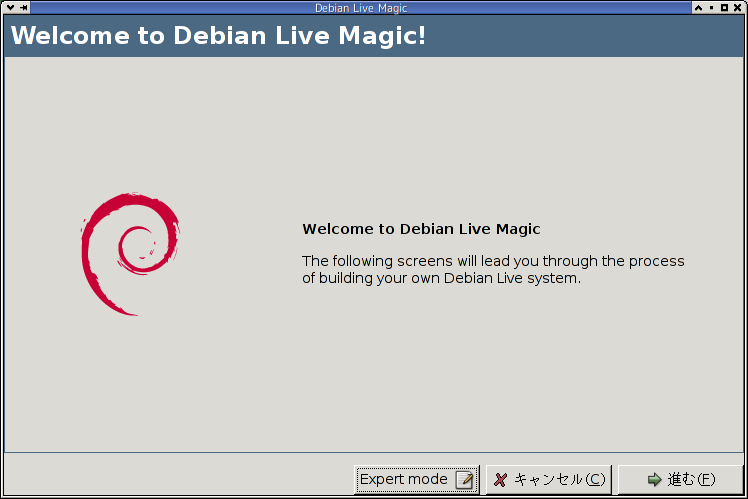
\includegraphics[width=1\hsize]{image200711/live-magic00.png}
 \end{center}
 \caption{live-magic 起動画面}
 \label{live-magic00}
 \end{figure}
\end{multicols}


\subsubsection{基本システムの選択}
次に基本システムを選択します。選択可能なシステムは以下の通りです。

\begin{multicols}{2}
 \begin{itemize}
 \item Gnome
 \item KDE
 \item XFCE
 \item non-Desktop
 \item システム復旧用 
 \end{itemize}

 \begin{figure}[H]
 \begin{center}
  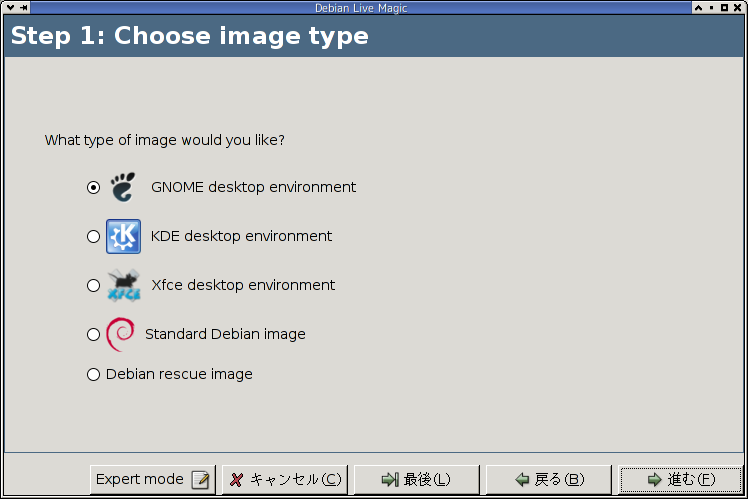
\includegraphics[width=1\hsize]{image200711/live-magic01.png}
 \end{center}
 \caption{live-magic 基本システムの選択}
 \label{live-magic01}
 \end{figure}
\end{multicols}

\subsubsection{作成イメージの選択}
次に作成するイメージを選択します。選択可能なイメージは以下の通りです。

\begin{multicols}{2}
 \begin{itemize}
 \item CD-ROM イメージ
 \item HDD イメージ
 \item NFS イメージ 
 \end{itemize}

 \begin{figure}[H]
 \begin{center}
  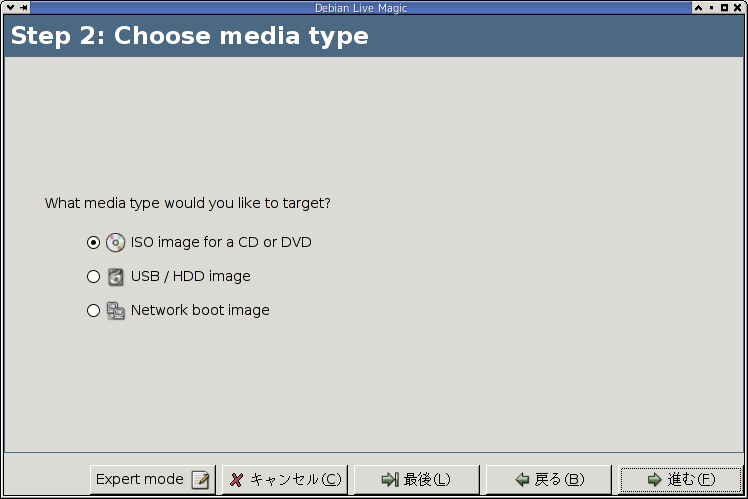
\includegraphics[width=1\hsize]{image200711/live-magic02.png}
 \end{center}
 \caption{live-magic 作成イメージの選択}
 \label{live-magic02}
 \end{figure}
\end{multicols}

\subsubsection{アーキテクチャの選択}
次に対象のアーキテクチャを選択します。選択可能なアーキテクチャは以下の通りです。

\begin{multicols}{2}
 \begin{itemize}
 \item i386
 \item powerpc
 \item amd64 
 \end{itemize}

 \begin{figure}[H]
 \begin{center}
  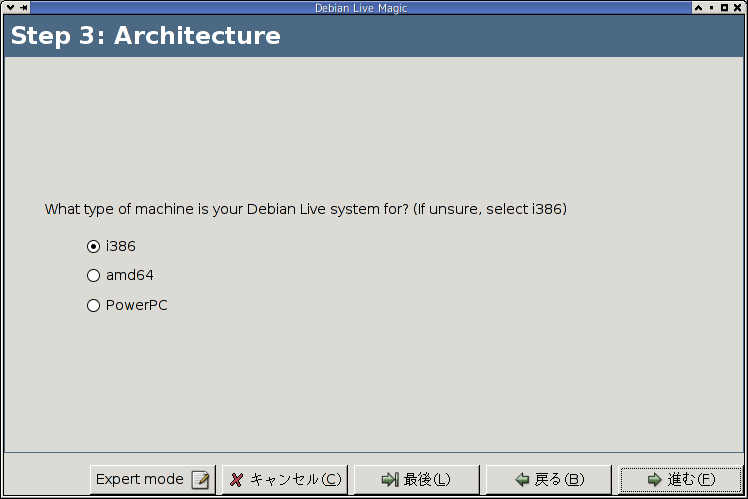
\includegraphics[width=1\hsize]{image200711/live-magic03.png}
 \end{center}
 \caption{live-magic アーキテクチャの選択}
 \label{live-magic03}
 \end{figure}
\end{multicols}

\subsubsection{ミラーサーバーの選択}
\begin{multicols}{2}
 次にミラーサーバーを選択します。

 \begin{figure}[H]
 \begin{center}
  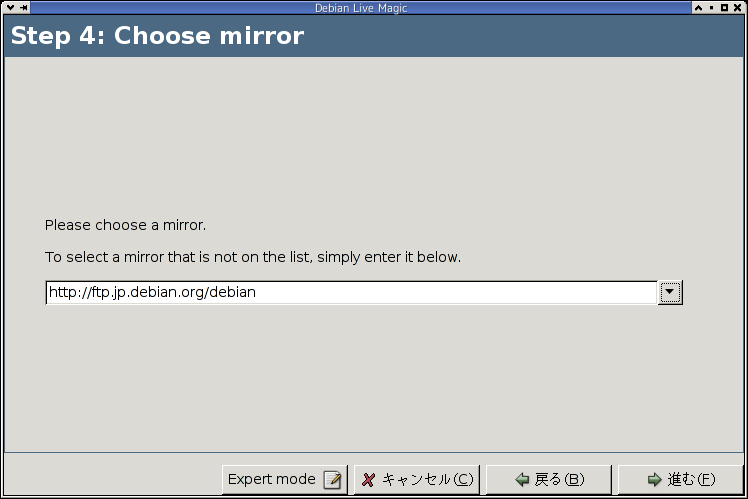
\includegraphics[width=1\hsize]{image200711/live-magic04.png}
 \end{center}
 \caption{live-magic ミラーサーバーの選択}
 \label{live-magic04}
 \end{figure}
\end{multicols}

\subsubsection{イメージ作成実行}
\begin{multicols}{2}
 適用ボタンを押すと、イメージ作成を実行します。

 \begin{figure}[H]
 \begin{center}
  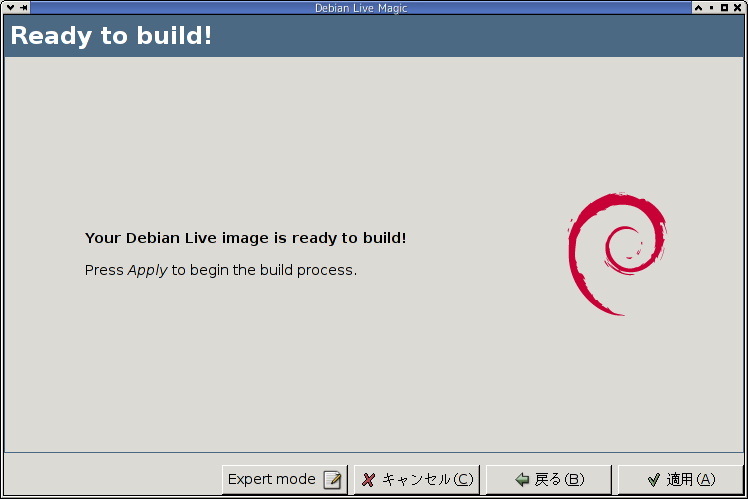
\includegraphics[width=1\hsize]{image200711/live-magic05.png}
 \end{center}
 \caption{live-magic イメージ作成実行}
 \label{live-magic05}
 \end{figure}
\end{multicols}


\subsubsection{rootパスワード要求}

\begin{multicols}{2}
 一般ユーザーで実行した場合、 rootのパスワードを要求されます。

 \begin{figure}[H]
 \begin{center}
  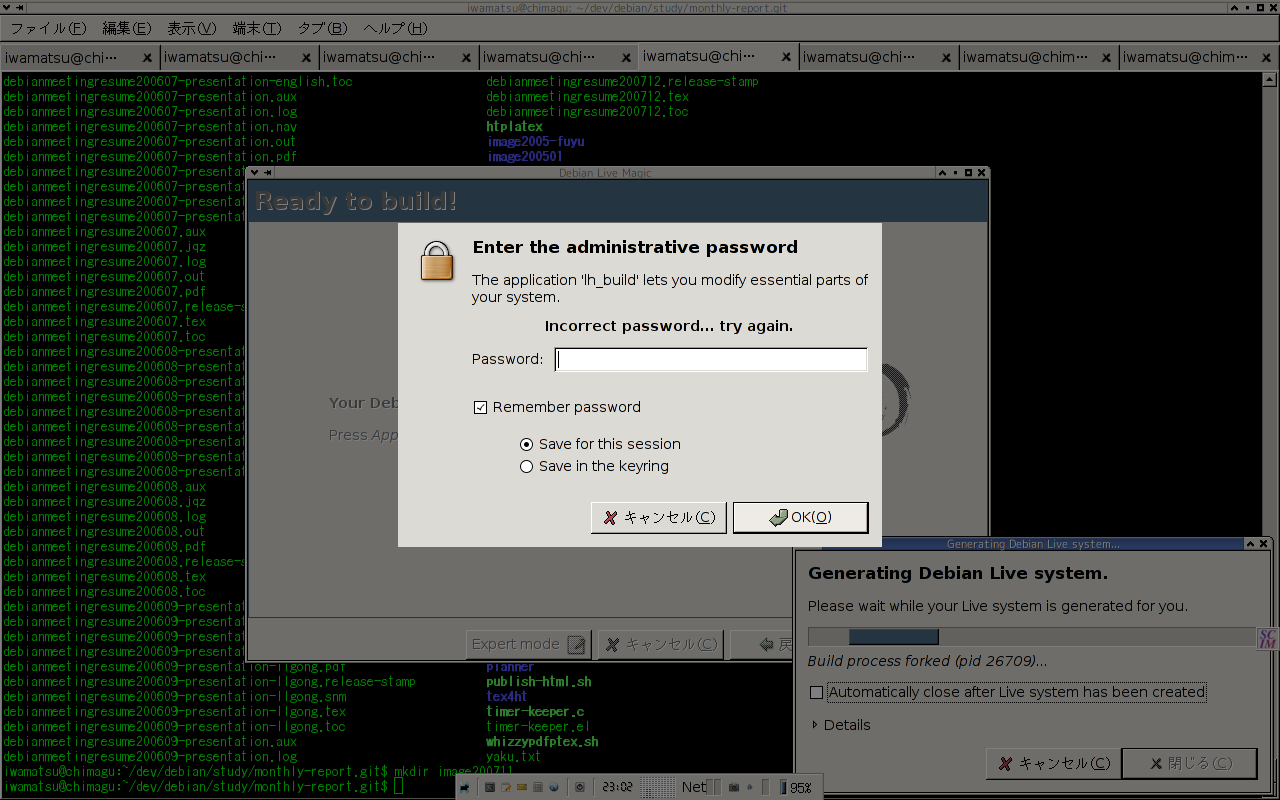
\includegraphics[width=1\hsize]{image200711/live-magic06.png}
 \end{center}
 \caption{live-magic rootパスワード要求画面}
 \label{live-magic06}
 \end{figure}
\end{multicols}

\subsubsection{作成中画面}

\begin{multicols}{2}
 イメージ作成中はプログレスバーが表示され、途中経過を確認することができます。

 \begin{figure}[H]
 \begin{center}
  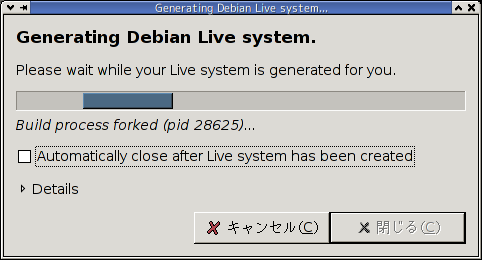
\includegraphics[width=1\hsize]{image200711/live-magic07.png}
 \end{center}
 \caption{live-magic 作成中画面}
 \label{live-magic07}
 \end{figure}
\end{multicols}

\subsubsection{デバッグ方法}
動作確認やデバッグのために、毎回作成した CD/DVD ISO イメージを 焼いていると
時間もお金もかかりますので、作成した ISO イメージのデバッグ方法について簡単に説
明したいと思います。

デバッグ方法はいろいろありますが、自分はqemu\footnote{http://packages.debian.org/sid/qemu}を使って動作確認しています。
\begin{commandline}
# apt-get update
# apt-get install qemu
% qemu -cdrom binary.iso
\end{commandline}
qemu を使ったエミュレーション環境でデバッグすることにより、時間や CD-R 代の節約にもなります。
他の方法としては、VMWare,VirtualPC を使ったデバッグ方法なども考えられます。

\subsection{live-helper を使ってみて}
\subsubsection{Live-CDからのインストールのサポート}
現状、Live-CD からのインストールがサポートされていません。
HDDイメージを作成することはできますが、一般ユーザーには敷居が高いと考えています。
Live-CD が気に入ったなら、動作している PC にインストールが容易にできるようになれば
ユーザーは増えるのではないでしょうか。

\subsubsection{日本語環境のサポート}
live-helper には、ある程度の環境をまとめたものとして、
packages-selections というものが提供されています。
これに日本語環境もサポートに入れることによって、日本語対応の Live-CD 作成が容易
になると思います。

\subsubsection{live-magic の日本語化}
live-helper のフロントエンドである live-magic が英語のままなので、国際化をしたい
ところです。


\subsection{その他の情報}
live-helper の情報は以下のサイトから得ることができます。
\begin{enumerate}
\item live-helper 公式サイト \url{http://debian-live.alioth.debian.org/}
\item wiki.debian.org \url{http://wiki.debian.org}

\end{enumerate}

\dancersection{HP ML350G5 Debian etch 動作確認}{上川 純一}
\label{ml350g5}
\index{ML350G5}

\subsection{サーバ}

HP ML350G5 は Intel Xeon CPUを搭載している
Debian 4.0 (etch) が稼働することがハードウェアベンダ、およびDebianプロジェ
クトの有志によって確認されているサーバ
\footnote{HP の ProLiant のDebian GNU/Linux 対応ページ:
\url{http://www.hp.com/go/debian}}
\footnote{Debian の ProLiant on Debian ページ:
\url{http://wiki.debian.org/HP/ProLiant}}
です。
今回利用したサーバには300GBのSASディスクが6本搭載されていました。

\subsection{インストール前の準備}

サーバの起動時に「F8」を押し、
ハードウェアRAID機能の設定を行います。
今回は一つのRAID5のボリューム(約1.5TB)としてOSに見せる設定にしました。

\subsection{インストール}

Debian installer でインストールします。今回はDebian GNU/Linux 4.0r1 DVD 
の1枚目を利用しました。ML350G5 は em64t 対応の Xeon のため、i386 でも 
amd64 でも動作します。今回は amd64 をインストールしました。

\subsection{デバイスの認識}

各種デバイスは簡単に稼働します。
グラフィックカードは ati ドライバで動作します。
debconf で自動設定した値で適切な設定ファイルが出力されます。

\begin{commandline}
# dpkg-reconfigure xserver-xorg
\end{commandline}

\subsection{USB ストレージデバイスの認識}


手元にあった「Green house GH-UFD2GR」のUSBメモリで動作確認したところ、認
識しました。

dmesg は次のようになりました:

 \begin{commandline}
 usb 6-6: new high speed USB device using ehci_hcd and address 4
 usb 6-6: configuration #1 chosen from 1 choice
 Initializing USB Mass Storage driver...
 scsi0 : SCSI emulation for USB Mass Storage devices
 usbcore: registered new driver usb-storage
 USB Mass Storage support registered.
 usb-storage: device found at 4
 usb-storage: waiting for device to settle before scanning
  Vendor: USBDisk   Model: FlashDisk         Rev: 1.00
  Type:   Direct-Access                      ANSI SCSI revision: 02
 usb-storage: device scan complete
 SCSI device sda: 4005000 512-byte hdwr sectors (2051 MB)
 sda: Write Protect is off
 sda: Mode Sense: 0b 00 00 08
 sda: assuming drive cache: write through
 SCSI device sda: 4005000 512-byte hdwr sectors (2051 MB)
 sda: Write Protect is off
 sda: Mode Sense: 0b 00 00 08
 sda: assuming drive cache: write through
 sda: sda1
 sd 0:0:0:0: Attached scsi removable disk sda
 \end{commandline}

df で確認しても認識されているのがわかります:

\begin{commandline}
# df -h /media/usbdisk/
Filesystem            Size  Used Avail Use% Mounted on
/dev/sda1             2.0G   76M  1.9G   4% /media/usbdisk
# df -T /media/usbdisk/
Filesystem    Type   1K-blocks      Used Available Use% Mounted on
/dev/sda1     vfat     2001888     76864   1925024   4% /media/usbdisk
\end{commandline}

\subsection{USB webcam の認識}

\begin{multicols}{2}

 PlayStation2 用USBカメラ EyeToy を動作させてみました。ov51x-jpeg のデバイ
 スドライバを認識させるためのドライバは残念ながらDebian 4.0 には含まれてい
 ないので、最新のドライバをバックポートしてみました。

 まず、インストールされたカーネルでコンパイルするために必要なパッケージを
 インストールします。

   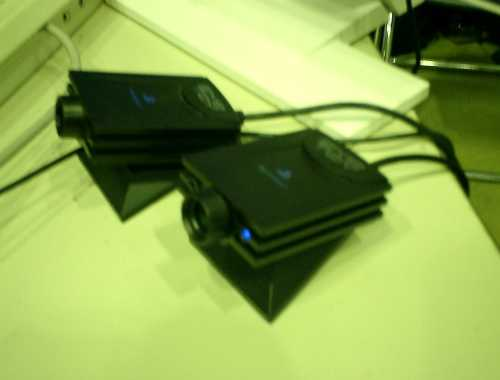
\includegraphics[width=0.8\hsize]{image200710/eyetoy.jpg}

\end{multicols}

\begin{commandline}
apt-get install linux-headers-2.6.18-5-amd64 linux-kbuild-2.6.18 \
 linux-source-2.6.18
\end{commandline}

ov51x-jpeg のソースを取得して make コマンドでビルドできます。

\begin{commandline}
debian:/home/hoge/ov51x-jpeg# make 
make -C /lib/modules/2.6.18-5-amd64/build M=/home/hoge/ov51x-jpeg modules
make[1]: Entering directory `/usr/src/linux-headers-2.6.18-5-amd64'
[中略]
make[1]: Leaving directory `/usr/src/linux-headers-2.6.18-5-amd64'
 
\end{commandline}

生成されたモジュールをあわせて insmod すれば ekiga で画面が見れるようになります。

\begin{commandline}
insmod v4l1-compat.ko
insmod v4l2-common.ko
insmod videodev.ko
insmod ov51x-jpeg.ko
\end{commandline}

\subsection{謝辞}

OSC Tokyo/Fall 2007 Debian ブースにて本作業を行いました。
サーバは日本HPからお借りしました。

\dancersection{HP ML110G4 Debian etch 動作確認}{上川 純一}
\label{ML110G4}
\index{ML110G4}

\subsection{サーバ}

HP の ML110G4 は Celeron CPU を搭載したサーバモデルです。今回利用したサー
バは SATA 接続のディスクを搭載していました。このハードウェア上でDebian
etch 4.0r1 が動作することは有志により確認されています\footnote{Debian の
ProLiant on Debian ページ: \url{http://wiki.debian.org/HP/ProLiant}}。ベ
ンダーとしては特に Debian の動作確認はしていないようです。

\subsection{インストール前の準備}

特に必要ないようです。

\subsection{インストール}

Debian installer でインストールします。今回はDebian GNU/Linux 4.0r1 DVD 
の1枚目を利用しました。i386 のインストールCDを利用しました。

\subsection{デバイスの認識}

グラフィックデバイスを自動認識できず、VESAモードで動作します。MGAのカー
ドなので、 mga ドライバで動作します。メモリが少ないため、デフォルトでは 
640x480x24 で動作するため若干画面が狭いです。 色を 16bit に減らすと 
1024x768x16 で動作しました。

\begin{commandline}
 SZ:    Pixels          Physical       Refresh
*0   1024 x 768    ( 271mm x 203mm )  *60  
 1    800 x 600    ( 271mm x 203mm )   75   72   60   56  
[略]
\end{commandline}

\subsection{謝辞}

OSC Tokyo/Fall 2007 Debian ブースにて本作業を行いました。
サーバはびぎねっとからお借りしました。


% \dancersection{今後の予定}{上川 純一}

% 12月15日に第35回東京エリア Debian 勉強会として忘年会を開催します。一年間
% の総括と、今後の進め方について議論します。

% 12月9日に第9回関西Debian勉強会が開催される予定です。

%\printindex

\cleartooddpage

\begin{minipage}[b]{0.2\hsize}
 \colorbox{dancerlightblue}{\rotatebox{90}{\fontsize{80}{80} {\gt デビアン勉強会} }}
\end{minipage}
\begin{minipage}[b]{0.8\hsize}

\vspace*{15cm}
{\color{dancerlightblue}\rule{\hsize}{1mm}}
\vspace{2mm}

\includegraphics[width=2cm]{image200502/openlogo-nd.eps}
\noindent \Large \bf Debian 勉強会資料\\ \\
\noindent \normalfont \debmtgyear{}年\debmtgmonth{}月\debmtgdate{}日 \hspace{5mm}  初版第1刷発行\\
\noindent \normalfont 東京エリア Debian 勉強会 (編集・印刷・発行)\\
{\color{dancerdarkblue}\rule{\hsize}{1mm}}
\end{minipage}

\end{document}
